\documentclass[usenames,dvipsnames]{beamer}

\usepackage{default}
\usepackage{tikz}
\usetikzlibrary{backgrounds}
\usetikzlibrary{arrows}

\usepackage{algorithm}
\usepackage{algpseudocode}
\usepackage{algorithmicx}

\usetheme{Berlin}

%%%%%%%%%%%%%% GENERAL %%%%%%%%%%%%%%
\newcommand{\ct}{\sim}

\newcommand{\ms}[1]{\overset{#1}{\leftarrow}}
\newcommand{\mt}[1]{\overset{#1}{\rightarrow}}

%%%%%%%%%%%%%% GG %%%%%%%%%%%%%%
\newcommand{\neigh}[1]{\operatorname{neigh}_{#1}}
\newcommand{\isomorph}{\cong}
\newcommand{\scont}[2]{\eta_{#1}(#2)}
\newcommand{\cont}[2]{\operatorname{cont}_{#1}(#2)}
\newcommand{\emb}[1]{\operatorname{emb}(#1)}
\newcommand{\allgraphs}[1]{\mathcal{G}_{#1}}
\newcommand{\startG}[1]{Z_{#1}}
\newcommand{\pro}{\to}

%%%%%%%%%%%%%% TGG %%%%%%%%%%%%%%
\newcommand{\alltgraphs}[1]{\mathcal{TG}_{#1}}
\newcommand{\startTG}[1]{Z_{#1}}
\newcommand{\emptyTG}{\varepsilon}
\newcommand{\source}{\operatorname{s}}
\newcommand{\Source}{\operatorname{S}}
\newcommand{\target}{\operatorname{t}}
\newcommand{\Target}{\operatorname{T}}
\newcommand{\cderiv}[3]{
	\ifx\relax#2\relax%
	\overset{#1}{\Rrightarrow}_{#3}%
	\else
	\overset{#1,#2}{\Rrightarrow}_{#3}%
	\fi
}
\newcommand{\deriv}[3]{
	\ifx\relax#2\relax
	\overset{#1}{\Rightarrow}_{#3}
	\else
	\overset{#1,#2}{\Rightarrow}_{#3}
	\fi
}
\newcommand{\derivtr}[1]{
	\Rightarrow^*_{#1}
}
\newcommand{\tcderiv}[3]{
	\ifx\relax#2\relax
	\overset{#1}{\Rrightarrow}_{#3}
	\else
	\overset{#1,#2}{\Rrightarrow}_{#3}
	\fi
}
\newcommand{\tderiv}[3]{
	\ifx\relax#2\relax
	\overset{#1}{\Rightarrow}_{#3}
	\else
	\overset{#1,#2}{\Rightarrow}_{#3}
	\fi
}
\newcommand{\tderivtr}[1]{\Rightarrow^*_{#1}}

%%%% PAC %%%%
\newcommand{\cderivpac}[4]{\overset{#1,#2,#3}{\Rrightarrow}_{#4}}
\newcommand{\derivpac}[4]{
	\ifx\relax#3\relax
	\overset{#1,#2}{\Rightarrow}_{#4}
	\else
	\overset{#1,#2,#3}{\Rightarrow}_{#4}
	\fi}
\newcommand{\derivpacn}[2]{\Rightarrow^{#2}_{#1}}
\newcommand{\resolv}[1]{\overset{#1}{\rightarrowtail}}
\newcommand{\resolvn}[2]{\overset{#1}{\rightarrowtail}^{#2}}
\newcommand{\derivpactr}[1]{\Rightarrow^*_{#1}}
\newcommand{\resolvtr}[1]{\rightarrowtail^*}

\newcommand{\tcderivpac}[4]{\overset{#1,#2,#3}{\Rrightarrow}_{#4}}
\newcommand{\tderivpac}[4]{
	\ifx\relax#3\relax
	\overset{#1,#2}{\Rightarrow}_{#4}
	\else
	\overset{#1,#2,#3}{\Rightarrow}_{#4}
	\fi
}
\newcommand{\tderivpacn}[2]{\Rightarrow^{#2}_{#1}}
\newcommand{\tresolv}[1]{\overset{#1}{\rightarrowtail}}
\newcommand{\tresolvn}[2]{\overset{#1}{\rightarrowtail}^{#2}}
\newcommand{\tderivpactr}[1]{\Rightarrow^*_{#1}}
\newcommand{\tresolvtr}[1]{\rightarrowtail^*_{#1}}



%%%%%%%%%%%%%% TIKZ %%%%%%%%%%%%%%
\tikzstyle{grammar}=[shorten >= 1pt, ->, draw=black!50, framed, background rectangle/.style={draw, rounded corners}, font=\scriptsize ]
\tikzstyle{graph}=[shorten >= 1pt, ->, draw=black!50, font=\scriptsize]
\tikzstyle{rid} = [inner sep=3pt, align=left, anchor=east]
\tikzstyle{nont}=[rectangle, inner sep=3pt, draw, fill=white, minimum width=5pt]
\tikzstyle{t}=[circle, inner sep=1pt, draw, fill=white, minimum width=5pt]
\tikzstyle{pac}=[circle, inner sep=1pt, draw, dotted, fill=white, minimum width=5pt]
\tikzstyle{empty}=[font=\Large, fill=white]
\tikzstyle{g}=[inner sep=3pt, fill=white]
\tikzstyle{lhs}=[inner sep=1pt, fill=white]
\tikzstyle{w}=[circle, inner sep=1pt, below=8pt, draw, fill=white, font=\tiny]
\tikzstyle{uw}=[circle, inner sep=1pt, above=8pt, draw, fill=white, font=\tiny]
\tikzstyle{edge}=[->, thin, -latex]
\tikzstyle{pacedge}=[->, thin, -latex, dotted]
\tikzstyle{edgeLabel}=[midway, above]
\tikzstyle{vledgeLabel}=[midway, left]
\tikzstyle{vredgeLabel}=[midway, right]
\tikzstyle{vbedgeLabel}=[above=3pt]
\tikzstyle{wedge}=[-, thin]
\tikzstyle{biedge}=[-, thin]
\tikzstyle{pipe}=[-, thick]
\tikzstyle{morph}=[-, thin, dashed, -latex]

\newcommand{\ridX}{-0.3}
\newcommand{\ridY}{0.5}
\newcommand{\lhsX}{-0.3}
\newcommand{\pipeUY}{-0.5}
\newcommand{\pipeBY}{0.5}

%% Scheme %%
\tikzstyle{scheme}=[shorten >= 1pt, ->, draw=black!50, framed, background rectangle/.style={draw, rounded corners}, font=\scriptsize ]
\tikzstyle{object}=[rectangle, inner sep=3pt, draw, fill=white, minimum width=5pt]
\tikzstyle{metaobject}=[rectangle, inner sep=3pt, draw, dashed, fill=white, minimum width=5pt]
\tikzstyle{activity}=[rectangle, inner sep=3pt, draw, fill=white, minimum width=5pt, rounded corners]

%Header Settings
\setbeamertemplate{headline}{}

%Footer Settings
\setbeamertemplate{navigation symbols}{
	\usebeamerfont{footline}%
	\usebeamercolor[fg]{footline}%
	\hspace{1em}%
	\insertframenumber/\inserttotalframenumber
}

\title[Model Transformation with TGG and Non-terminal Symbols]{Model Transformation with Triple Graph Grammars and Non-terminal Symbols}
\author[W. da Silva et al.]{William da Silva, Max Bureck, Ina Schieferdecker, and Christian Hein}
\institute[Fraunhofer Fokus]
{
	\vskip 12pt
	Fraunhofer Fokus, Berlin, Germany \\
	\texttt{william.bombardelli.da.silva@fokus.fraunhofer.de}\\
	Technische Universit\"{a}t Berlin, Berlin, Germany
}
\date{November 2, 2018}

\makeatletter
\hypersetup{
	pdftitle = {\@title}, pdfkeywords = {Model Transformation}, pdfauthor = {\@author}
} 
\makeatother

\begin{document}
	\begin{frame}
		\titlepage
	\end{frame}
	
	\begin{frame}
		\frametitle{Organization}
		\tableofcontents
	\end{frame}
	
	%-------------------
	% Introcudtion
	%-------------------
	\section{Introduction}
	\begin{frame}
		\frametitle{Introduction}
		\tableofcontents[currentsection, currentsubsection] 
	\end{frame}
	
	\begin{frame}{Background}
		\begin{itemize}
			\item Model-driven software development as a technique to enhance quality of software
			\pause
			\item Models as formal specifications of safety-critical systems
			\pause
			\item Transformation between models (e.g. from a formal specification to high-level source-code and vice-versa)
			\pause
			\medskip
			\item \textbf{Goal:} Comprehensible and reliable transformations
			\begin{itemize}
				\item Efficient representation of abstract concepts
				\item Small size
			\end{itemize}
		\end{itemize}
	\end{frame}
	
	\begin{frame}{The Model Transformation Problem}
		\centering{
		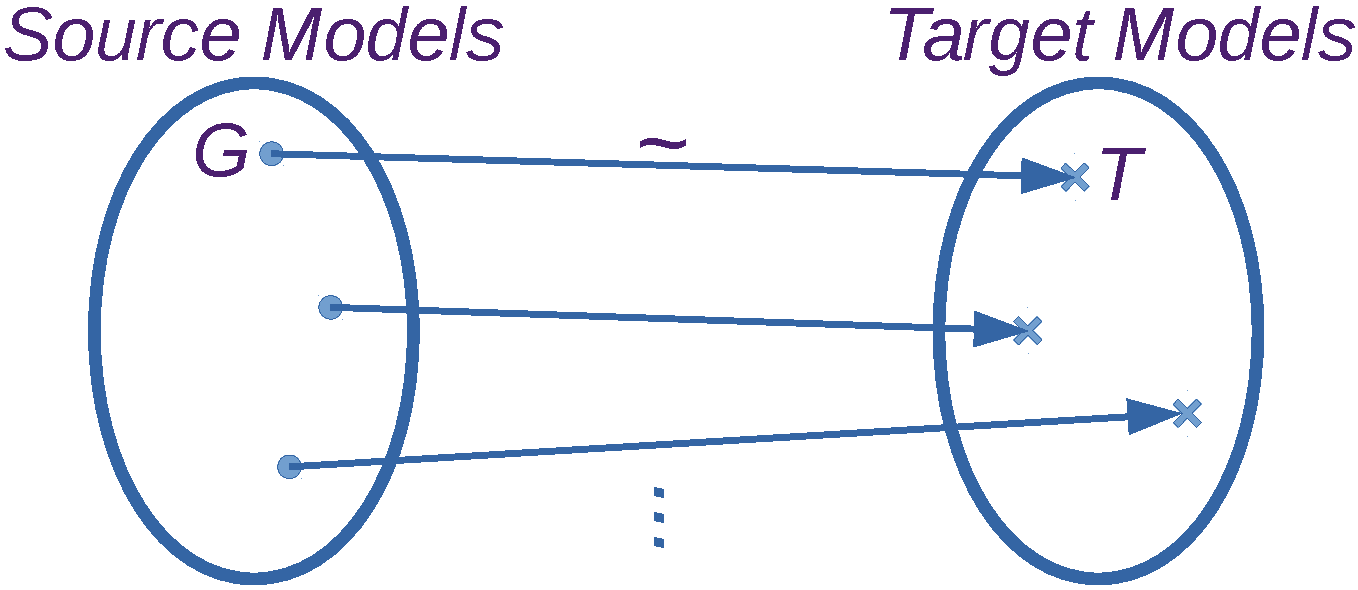
\includegraphics[width=.7\textwidth]{misc/model-transformation}
		}
		\begin{itemize}
			\item $G \ct T$ iff $G$ is correctly transformed into $T$
			\item $\ct$ is the \emph{correctly-transformed relation} between source and target models
			\item \textbf{Batch forward transformation:} \\
			Given $G$, find a $T$, such that $G \ct T$
		\end{itemize}
		
	\end{frame}
	
	\begin{frame}{The Triple Graph Grammar Approach}
		\begin{itemize}
			\item Models are graphs
			\pause
			\item Two correctly-transformed graphs $G$ and $T$ are in a triple graph $G \ms{} C \mt{} T$\\
				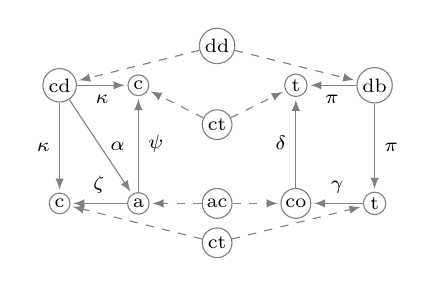
\begin{tikzpicture}[graph]
	\draw (1,0) node[t] (s1) {cd};
	\draw (1,-1.5) node[t] (s2) {c};
	\draw (2,-1.5) node[t] (s4) {a};
	\draw (2,0) node[t] (s5) {c};
	\draw[edge] (s1) -- (s2) node [vledgeLabel] {$\kappa$};
	\draw[edge] (s1) -- (s4) node [vredgeLabel] {$\alpha$};
	\draw[edge] (s1) -- (s5) node [edgeLabel, below] {$\kappa$};
	\draw[edge] (s4) -- (s2) node [edgeLabel] {$\zeta$};
	\draw[edge] (s4) -- (s5) node [vredgeLabel] {$\psi$};
	%
	\draw (3,0.5) node[t] (c1) {dd};
	\draw (3,-2) node[t] (c2) {ct};
	\draw (3,-1.5) node[t] (c4) {ac};
	\draw (3,-0.5) node[t] (c5) {ct};
	%
	\draw (5,0) node[t] (t1) {db};
	\draw (5,-1.5) node[t] (t2) {t};
	\draw (4,-1.5) node[t] (t4) {co};
	\draw (4,0) node[t] (t5) {t};
	\draw[edge] (t1) -- (t2) node [vredgeLabel] {$\pi$};
	\draw[edge] (t1) -- (t5) node [edgeLabel, below] {$\pi$};
	\draw[edge] (t2) -- (t4) node [edgeLabel] {$\gamma$};
	\draw[edge] (t4) -- (t5) node [vledgeLabel] {$\delta$};
	%
	\draw[morph] (c1) -- (s1);
	\draw[morph] (c1) -- (t1);
	\draw[morph] (c2) -- (s2);
	\draw[morph] (c2) -- (t2);
	\draw[morph] (c4) -- (s4);
	\draw[morph] (c4) -- (t4);
	\draw[morph] (c5) -- (s5);
	\draw[morph] (c5) -- (t5);
	\end{tikzpicture}

			\pause
			\item A triple graph grammar $TGG$ is a generator of a set of triple graphs $L(TGG)$
			\pause
			\item The correctly-transformed relation $\ct$ between graphs is described in terms of a triple graph grammar $TGG$
			\begin{itemize}
				\item $G \ct T $ iff $(G \ms{} C \mt{} T) \in L(TGG)$
			\end{itemize}
		\end{itemize}
	\end{frame}
	
	\begin{frame}{TGG -- An Example}
		\begin{itemize}
			\item \emph{Pseudocode} to \emph{Controlflow}
		\end{itemize}
		
		\begin{minipage}[h]{.48\textwidth}
	\begin{algorithmic}[!ht]
		\State \Program $main(n)$
		\If {$n < 0$}
			\State \Return $\Nothing$
		\Else
			\State $f \gets 1$ 
			\While {$n > 0$}
				\State $f \gets f * n$
				\State $n \gets n - 1$
			\EndWhile
			\State \Return $\Just f$
		\EndIf
	\end{algorithmic}
\end{minipage}
\begin{minipage}[h]{.5\textwidth}
	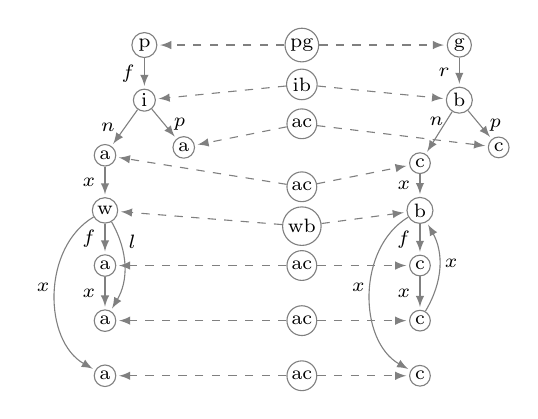
\begin{tikzpicture}[graph]
	\draw (1,0) node[t] (s1) {p};
	\draw (1,-0.7) node[t] (s2) {i};
	\draw (1.5,-1.3) node[t] (s3) {a};
	\draw (0.5,-1.4) node[t] (s4) {a};
	\draw (0.5,-2.1) node[t] (s5) {w};
	\draw (0.5,-2.8) node[t] (s6) {a};
	\draw (0.5,-3.5) node[t] (s7) {a};
	\draw (0.5,-4.2) node[t] (s8) {a};
	
	\draw[edge] (s1) -- (s2) node [vledgeLabel] {$f$};
	\draw[edge] (s2) -- (s3) node [vredgeLabel] {$p$};
	\draw[edge] (s2) -- (s4) node [vledgeLabel] {$n$};
	\draw[edge] (s4) -- (s5) node [vledgeLabel] {$x$};
	\draw[edge] (s5) -- (s6) node [vledgeLabel] {$f$};
	\draw[edge] (s5) to [bend left] (s7) node [above=25pt, right=3pt] {$l$};
	\draw[edge] (s5) to [bend right=60] (s8) node [above=30pt, left=13pt] {$x$};
	\draw[edge] (s6) -- (s7) node [vledgeLabel] {$x$};
	%
	\draw (3,0) node[t] (c1) {pg};
	\draw (3,-0.5) node[t] (c2) {ib};
	\draw (3,-1.0) node[t] (c3) {ac};
	\draw (3,-1.8) node[t] (c4) {ac};
	\draw (3,-2.3) node[t] (c5) {wb};
	\draw (3,-2.8) node[t] (c6) {ac};
	\draw (3,-3.5) node[t] (c7) {ac};
	\draw (3,-4.2) node[t] (c8) {ac};
	%
	\draw (5,0) node[t] (t1) {g};
	\draw (5,-0.7) node[t] (t2) {b};
	\draw (5.5,-1.3) node[t] (t3) {c};
	\draw (4.5,-1.5) node[t] (t4) {c};
	\draw (4.5,-2.1) node[t] (t5) {b};
	\draw (4.5,-2.8) node[t] (t6) {c};
	\draw (4.5,-3.5) node[t] (t7) {c};
	\draw (4.5,-4.2) node[t] (t8) {c};
	
	\draw[edge] (t1) -- (t2) node [vledgeLabel] {$r$};
	\draw[edge] (t2) -- (t3) node [vredgeLabel] {$p$};
	\draw[edge] (t2) -- (t4) node [above=15pt, right=0pt] {$n$};
	\draw[edge] (t4) -- (t5) node [vledgeLabel] {$x$};
	\draw[edge] (t5) -- (t6) node [vledgeLabel] {$f$};
	\draw[edge] (t7) to [bend right] (t5) node [below=15pt, right=3pt] {$x$};
	\draw[edge] (t5) to [bend right=60] (t8) node [above=30pt, left=13pt] {$x$};
	\draw[edge] (t6) -- (t7) node [vledgeLabel] {$x$};
	%
	\draw[morph] (c1) -- (s1);
	\draw[morph] (c1) -- (t1);
	\draw[morph] (c2) -- (s2);
	\draw[morph] (c2) -- (t2);
	\draw[morph] (c3) -- (s3);
	\draw[morph] (c3) -- (t3);
	\draw[morph] (c4) -- (s4);
	\draw[morph] (c4) -- (t4);
	\draw[morph] (c5) -- (s5);
	\draw[morph] (c5) -- (t5);
	\draw[morph] (c6) -- (s6);
	\draw[morph] (c6) -- (t6);
	\draw[morph] (c7) -- (s7);
	\draw[morph] (c7) -- (t7);
	\draw[morph] (c8) -- (s8);
	\draw[morph] (c8) -- (t8);
	\end{tikzpicture}
\end{minipage}%
	\end{frame}
	
	\begin{frame}{TGG - An Example}
		\begin{itemize}
			\item \emph{Pseudocode} to \emph{Controlflow}
		\end{itemize}
			
			\centering
	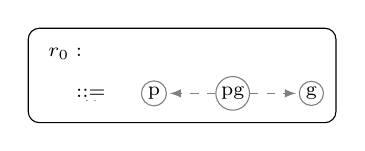
\begin{tikzpicture}[grammar]
	\node[rid] at (\ridX,\ridY) {$r_0:$};
	\draw (\lhsX,0) node[lhs] (lhs) {::=};
	
	\draw (0.5,0) node[t] (s1) {p};
	%%
	\draw (1.5,0) node[t] (c1) {pg};
	%%
	\draw (2.5,0) node[t] (t1) {g};
	%%
	\draw[morph] (c1) -- (s1);
	\draw[morph] (c1) -- (t1);
	\end{tikzpicture}
		
	\vskip 5pt
		
	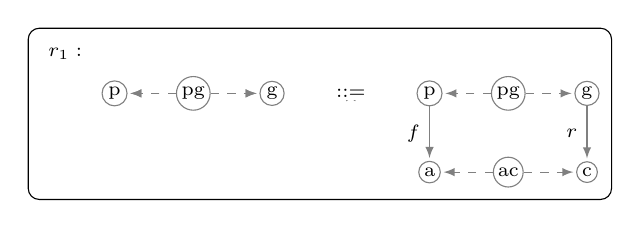
\begin{tikzpicture}[grammar]
	\node[rid] at (\ridX,\ridY) {$r_1:$};
	
	\draw (0,0) node[t] (s1) {p};
	%%
	\draw (1,0) node[t] (c1) {pg};
	%%
	\draw (2,0) node[t] (t1) {g};
	%%
	\draw[morph] (c1) -- (s1);
	\draw[morph] (c1) -- (t1);
	%%%%%%
	\draw (3,0) node[lhs] (lhs) {::=};
	%%%%%%	
	\draw (4,0) node[t] (s2) {p};
	\draw (4,-1) node[t] (s3) {a};
	\draw[edge] (s2) -- (s3) node [vledgeLabel] {$f$};
	%%
	\draw (5,0) node[t] (c2) {pg};
	\draw (5,-1) node[t] (c3) {ac};
	%%
	\draw (6,0) node[t] (t2) {g};
	\draw (6,-1) node[t] (t3) {c};
	\draw[edge] (t2) -- (t3) node [vledgeLabel] {$r$};
	%%
	\draw[morph] (c1) -- (s1);
	\draw[morph] (c1) -- (t1);
	\draw[morph] (c2) -- (s2);
	\draw[morph] (c2) -- (t2);
	\draw[morph] (c3) -- (s3);
	\draw[morph] (c3) -- (t3);
	\end{tikzpicture}
	
	\vskip 5pt
	
	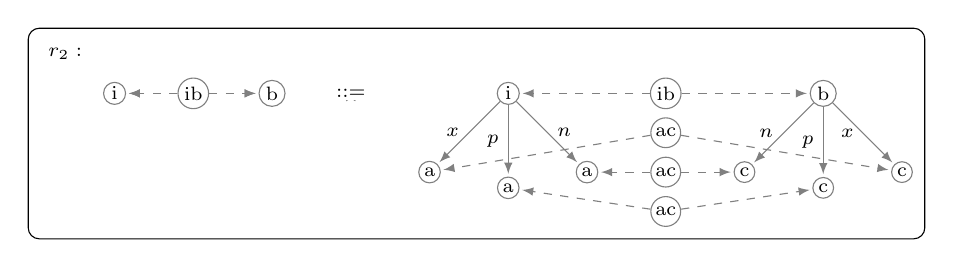
\begin{tikzpicture}[grammar]
	\node[rid] at (\ridX,\ridY) {$r_2:$};
	
	\draw (0,0) node[t] (s1) {i};
	%%
	\draw (1,0) node[t] (c1) {ib};
	%%
	\draw (2,0) node[t] (t1) {b};
	%%
	\draw[morph] (c1) -- (s1);
	\draw[morph] (c1) -- (t1);
	%%%%%%
	\draw (3,0) node[lhs] (lhs) {::=};
	%%%%%%
	\draw (5,0) node[t] (s2) {i};
	\draw (4,-1) node[t] (s3) {a};
	\draw (5,-1.2) node[t] (s4) {a};
	\draw (6,-1) node[t] (s5) {a};
	\draw[edge] (s2) -- (s3) node [vledgeLabel] {$x$};
	\draw[edge] (s2) -- (s4) node [vledgeLabel] {$p$};
	\draw[edge] (s2) -- (s5) node [vredgeLabel] {$n$};
	%%
	\draw (7,0) node[t] (c2) {ib};
	\draw (7,-0.5) node[t] (c3) {ac};
	\draw (7,-1.5) node[t] (c4) {ac};
	\draw (7,-1) node[t] (c5) {ac};
	%%
	\draw (9,0) node[t] (t2) {b};
	\draw (10,-1) node[t] (t3) {c};
	\draw (9,-1.2) node[t] (t4) {c};
	\draw (8,-1) node[t] (t5) {c};
	\draw[edge] (t2) -- (t3) node [vledgeLabel] {$x$};
	\draw[edge] (t2) -- (t4) node [vledgeLabel] {$p$};
	\draw[edge] (t2) -- (t5) node [vledgeLabel] {$n$};
	%%
	\draw[morph] (c1) -- (s1);
	\draw[morph] (c1) -- (t1);
	\draw[morph] (c2) -- (s2);
	\draw[morph] (c2) -- (t2);
	\draw[morph] (c3) -- (s3);
	\draw[morph] (c3) -- (t3);
	\draw[morph] (c4) -- (s4);
	\draw[morph] (c4) -- (t4);
	\draw[morph] (c5) -- (s5);
	\draw[morph] (c5) -- (t5);
	\end{tikzpicture}
	\end{frame}
	
	%-------------------
	%  TGG With Non-terminals
	%-------------------
	\section{Triple Graph Grammars with Non-terminal Symbols}
	\begin{frame}
		\frametitle{Triple Graph Grammars with Non-terminal Symbols}
		\tableofcontents[currentsection, currentsubsection] 
	\end{frame}
	
	\begin{frame}{Our Contribution -- NCE TGG}
		\begin{itemize}
			\item New formalism: NCE TGG
			\begin{itemize}
				\item \emph{Graph Grammar with Neighborhood-controlled Embedding} (NCE) \cite{janssens1982graph}
				\item \emph{Triple Graph Grammar} (TGG) \cite{schurr1994specification}
			\end{itemize}
			\item Non-terminal symbols
			\item Context-free
		\end{itemize}
	\end{frame}
	
	\begin{frame}{NCE TGG -- An Example}
		\begin{itemize}
			\item \emph{Pseudocode} to \emph{Controlflow}
		\end{itemize}
		
			\noindent
	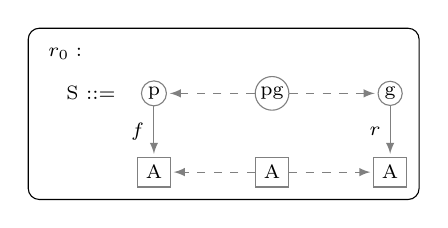
\begin{tikzpicture}[grammar]
	\node[rid] at (\ridX,\ridY) {$r_0:$};
	\draw (\lhsX,0) node[lhs] (lhs) {S ::=};
	
	\draw (0.5,0) node[t] (s1) {p};
	\draw (0.5,-1) node[nont] (s2) {A};
	\draw[edge] (s1) -- (s2) node [vledgeLabel] {$f$};
	%%
	\draw (2,0) node[t] (c1) {pg};
	\draw (2,-1) node[nont] (c2) {A};
	%%
	\draw (3.5,0) node[t] (t1) {g};
	\draw (3.5,-1) node[nont] (t2) {A};
	\draw[edge] (t1) -- (t2) node [vledgeLabel] {$r$};
	%%
	\draw[morph] (c1) -- (s1);
	\draw[morph] (c1) -- (t1);
	\draw[morph] (c2) -- (s2);
	\draw[morph] (c2) -- (t2);
	\end{tikzpicture}
	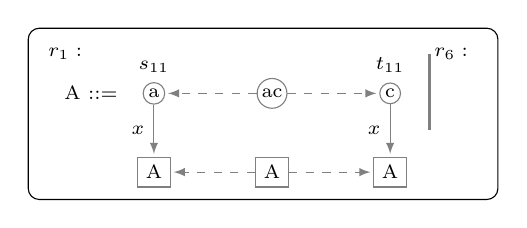
\begin{tikzpicture}[grammar]
	\node[rid] at (\ridX,\ridY) {$r_1:$};
	\draw (\lhsX,0) node[lhs] (lhs) {A ::=};
	
	\draw (0.5,0) node[t, label=90:$s_{11}$] (s1) {a};
	\draw (0.5,-1) node[nont] (s2) {A};
	\draw[edge] (s1) -- (s2) node [vledgeLabel] {$x$};
	%\draw node[uw] at (s1.east) (w-s1) {} [wedge] (s1) -- (w-s1);
	%%
	\draw (2,0) node[t] (c1) {ac};
	\draw (2,-1) node[nont] (c2) {A};
	%%
	\draw (3.5,0) node[t, label=90:$t_{11}$] (t1) {c};
	\draw (3.5,-1) node[nont] (t2) {A};
	\draw[edge] (t1) -- (t2) node [vledgeLabel] {$x$};
	%\draw node[uw] at (t1.north) (w-t1) {} [wedge] (t1) -- (w-t1);
	%%
	\draw[morph] (c1) -- (s1);
	\draw[morph] (c1) -- (t1);
	\draw[morph] (c2) -- (s2);
	\draw[morph] (c2) -- (t2);
	
	%%%%
	\draw[pipe] (4,\pipeBY) -- (4,\pipeUY);
	
	\node[rid] at (4.6,\ridY) {$r_6:$};
	\draw (4.6,0) node[empty] (s3) {$\emptyGraph$};
	\end{tikzpicture}
	
	\noindent
	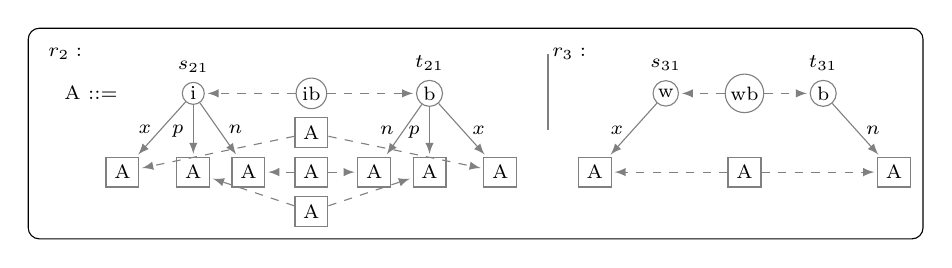
\begin{tikzpicture}[grammar]
	\node[rid] at (\ridX,\ridY) {$r_2:$};
	\draw (\lhsX,0) node[lhs] (lhs) {A ::=};
	
	\draw (1,0) node[t, label=90:$s_{21}$] (s1) {i};
	\draw (0.1,-1) node[nont] (s2) {A};
	\draw (1,-1) node[nont] (s3) {A};
	\draw (1.7,-1) node[nont] (s4) {A};
	\draw[edge] (s1) -- (s2) node [vledgeLabel] {$x$};
	\draw[edge] (s1) -- (s3) node [vledgeLabel] {$p$};
	\draw[edge] (s1) -- (s4) node [vredgeLabel] {$n$};
	%\draw node[uw] at (s1.north) (w-s1) {} [wedge] (s1) -- (w-s1);
	%%
	\draw (2.5,0) node[t] (c1) {ib};
	\draw (2.5,-0.5) node[nont] (c2) {A};
	\draw (2.5,-1) node[nont] (c4) {A};
	\draw (2.5,-1.5) node[nont] (c3) {A};
	%%
	\draw (4,0) node[t, label=90:$t_{21}$] (t1) {b};
	\draw (3.3,-1) node[nont] (t4) {A};
	\draw (4,-1) node[nont] (t3) {A};
	\draw (4.9,-1) node[nont] (t2) {A};
	\draw[edge] (t1) -- (t4) node [vledgeLabel] {$n$};
	\draw[edge] (t1) -- (t3) node [vledgeLabel] {$p$};
	\draw[edge] (t1) -- (t2) node [vredgeLabel] {$x$};
	%\draw node[uw] at (t1.north) (w-t1) {} [wedge] (t1) -- (w-t1);
	%%
	\draw[morph] (c1) -- (s1);
	\draw[morph] (c1) -- (t1);
	\draw[morph] (c2) -- (s2);
	\draw[morph] (c2) -- (t2);
	\draw[morph] (c3) -- (s3);
	\draw[morph] (c3) -- (t3);
	\draw[morph] (c4) -- (s4);
	\draw[morph] (c4) -- (t4);
	
	%%%%
	\draw[pipe] (5.5,\pipeBY) -- (5.5,\pipeUY);
	
	\node[rid] at (6.1,\ridY) {$r_3:$};
	
	\draw (7,0) node[t, label=90:$s_{31}$] (s5) {w};
	\draw (6.1,-1) node[nont] (s6) {A};
	\draw[edge] (s5) -- (s6) node [vledgeLabel] {$x$};
	%\draw node[uw] at (s5.north) (w-s5) {} [wedge] (s5) -- (w-s5);
	%%
	\draw (8,0) node[t] (c5) {wb};
	\draw (8,-1) node[nont] (c6) {A};
	%%
	\draw (9,0) node[t, label=90:$t_{31}$] (t5) {b};
	\draw (9.9,-1) node[nont] (t6) {A};
	\draw[edge] (t5) -- (t6) node [vredgeLabel] {$n$};
	%\draw node[uw] at (t5.north) (w-t5) {} [wedge] (t5) -- (w-t5);
	%%
	\draw[morph] (c5) -- (s5);
	\draw[morph] (c5) -- (t5);
	\draw[morph] (c6) -- (s6);
	\draw[morph] (c6) -- (t6);
	\end{tikzpicture}
	
	\noindent
	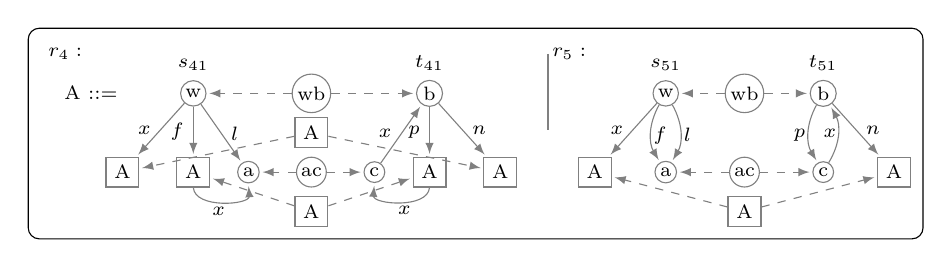
\begin{tikzpicture}[grammar]
	\node[rid] at (\ridX,\ridY) {$r_4:$};
	\draw (\lhsX,0) node[lhs] (lhs) {A ::=};
	
	\draw (1,0) node[t, label=90:$s_{41}$] (s1) {w};
	\draw (0.1,-1) node[nont] (s2) {A};
	\draw (1,-1) node[nont] (s3) {A};
	\draw (1.7,-1) node[t] (s4) {a};
	
	\draw[edge] (s1) -- (s2) node [vledgeLabel] {$x$};
	\draw[edge] (s1) -- (s3) node [vledgeLabel] {$f$};
	\draw[edge] (s3) to [bend right=90] (s4) node [below=10pt, left=5pt] {$x$};
	\draw[edge] (s1) -- (s4) node [vredgeLabel] {$l$};
	%\draw node[uw] at (s1.north) (w-s1) {} [wedge] (s1) -- (w-s1);
	%%
	\draw (2.5,0) node[t] (c1) {wb};
	\draw (2.5,-0.5) node[nont] (c2) {A};
	\draw (2.5,-1) node[t] (c4) {ac};
	\draw (2.5,-1.5) node[nont] (c3) {A};
	%%
	\draw (4,0) node[t, label=90:$t_{41}$] (t1) {b};
	\draw (3.3,-1) node[t] (t4) {c};
	\draw (4,-1) node[nont] (t3) {A};
	\draw (4.9,-1) node[nont] (t2) {A};
	\draw[edge] (t1) -- (t2) node [vredgeLabel] {$n$};
	\draw[edge] (t1) -- (t3) node [vledgeLabel] {$p$};
	\draw[edge] (t3) to [bend left=90] (t4) node [below=10pt, right=5pt] {$x$};
	\draw[edge] (t4) -- (t1) node [vledgeLabel] {$x$};
	%\draw node[uw] at (t1.north) (w-t1) {} [wedge] (t1) -- (w-t1);
	%%
	\draw[morph] (c1) -- (s1);
	\draw[morph] (c1) -- (t1);
	\draw[morph] (c2) -- (s2);
	\draw[morph] (c2) -- (t2);
	\draw[morph] (c3) -- (s3);
	\draw[morph] (c3) -- (t3);
	\draw[morph] (c4) -- (s4);
	\draw[morph] (c4) -- (t4);
	
	%%%%
	\draw[pipe] (5.5,\pipeBY) -- (5.5,\pipeUY);
	
	\node[rid] at (6.1,\ridY) {$r_5:$};
	
	\draw (7,0) node[t, label=90:$s_{51}$] (s5) {w};
	\draw (6.1,-1) node[nont] (s6) {A};
	\draw (7,-1) node[t] (s7) {a};
	\draw[edge] (s5) -- (s6) node [vledgeLabel] {$x$};
	\draw[edge] (s5) to [bend right] (s7) node [vbedgeLabel] {$f$};
	\draw[edge] (s5) to [bend left] (s7) node [above=10pt, right=1pt] {$l$};
	%\draw node[uw] at (s5.north) (w-s5) {} [wedge] (s5) -- (w-s5);
	%%
	\draw (8,0) node[t] (c5) {wb};
	\draw (8,-1.5) node[nont] (c6) {A};
	\draw (8,-1) node[t] (c7) {ac};
	%%
	\draw (9,0) node[t, label=90:$t_{51}$] (t5) {b};
	\draw (9,-1) node[t] (t7) {c};
	\draw (9.9,-1) node[nont] (t6) {A};
	\draw[edge] (t5) -- (t6) node [vredgeLabel] {$n$};
	\draw[edge] (t5) to [bend right] (t7) node [above=10pt, left=1pt] {$p$};
	\draw[edge] (t7) to [bend right] (t5) node [below=5pt] {$x$};
	%\draw node[uw] at (t5.north) (w-t5) {} [wedge] (t5) -- (w-t5);
	%%
	\draw[morph] (c5) -- (s5);
	\draw[morph] (c5) -- (t5);
	\draw[morph] (c6) -- (s6);
	\draw[morph] (c6) -- (t6);
	\draw[morph] (c7) -- (s7);
	\draw[morph] (c7) -- (t7);
	\end{tikzpicture}
	\end{frame}
	
	%TODO: FTSCS - Derivation Example
	
	%TODO: FTSCS - Transformation Discussion
	
	%-------------------
	%  Evaluation
	%-------------------
	\section{Evaluation}
	\begin{frame}
		\frametitle{Evaluation}
		\tableofcontents[currentsection, currentsubsection] 
	\end{frame}
	
	\begin{frame}{Usability Evaluation}
		\footnotesize 
		\begin{table}[h]
			\centering
			\begin{tabular}{l r r r r }
				\hline
				& \multicolumn{2}{c}{Standard TGG} & \multicolumn{2}{c}{BNCE TGG}\\
				Transformation 			& Rules & Elements 	& Rules & Elements\\
				\hline
				Pseudocode2Controlflow	& 47			& 1085	& \textbf{7}	& \textbf{185} \\
				BTree2XBTree			& \textbf{4}	& \textbf{50}	& 5		& 80 \\
				Star2Wheel				& -				& -		& \textbf{6}	& \textbf{89} \\
				Class2Database			& \textbf{5}	& \textbf{80}	& - 	& -  \\
				\hline
			\end{tabular}
			\caption{Results of the usability evaluation of the BNCE TGG formalism in comparison with the standard TGG for the model transformation problem}
		\end{table}
	\end{frame}
	
	%-------------------
	%  Conclusion
	%-------------------
	\section{Conclusion}
	\begin{frame}
		\frametitle{Conclusion}
		\tableofcontents[currentsection, currentsubsection] 
	\end{frame}
	
	\begin{frame}{Conclusion}
		\begin{itemize}
			\item New context-free TGG formalism
			\begin{itemize}
				\item Used to specify model transformations
				\item Outperforms standard TGG in 2 evaluated cases
				\item Special potential for code-generation
				\item Cannot model important transformations (e.g. Class Diagrams)
			\end{itemize}
			\pause
			\item Future Work
			\begin{itemize}
				\item Application conditions: Positive experimental results
				\item Broader evaluation including empirical assessment with engineers and performance reports
				\item Model synchronization
			\end{itemize}
		\end{itemize}
	\end{frame}
	
	%-------------------
	% References
	%-------------------
	\section{References}
	\begin{frame}
		\frametitle{References}
		\tableofcontents[currentsection, currentsubsection] 
	\end{frame}
	
	\begin{frame}
		\frametitle{References}
		\tiny
		\bibliographystyle{plainnat}
		\bibliography{bibliography}
	\end{frame}
\end{document}
